\chapter{Temporal logics and Linear Dynamic Logic}

\label{ch:logics}

\section{Temporal logics on finite traces}

% Intro to temporal logics
Temporal logics are a class of formal languages, more precisely modal logics,
that allow to talk about properties and events over
time~\cite{bib:temporal-logics-stanford}. Among all formalisms, we care about
logics that assume a linear time, as opposed to branching, and a discrete
sequence of instants, instead of continuous time.  In computer science, the
most famous logic in this group is the Pnueli's Linear Temporal Logic
(LTL)\nomenclature{LTL}{Linear Temporal Logic}~\cite{bib:pnueli-ltl}.

% Structures
The assumptions about the nature of time directly reflect to the type of
structures these logics are interpreted on: their models are tuples $\modelsym
= \langle T, \prec, V \rangle$, where $T$ is a discrete set of time instants,
such as $\N$, $\prec$ is a complete ordering relation on $T$, like~$<$, and
$V$ is a valuation function $V: T \times \fluents \to \{\true, \false\}$. For
a logic that defines a set $\fluents$ of proposition symbols, the function $V$
assigns a truth value to each of them, in every instant of time. The symbols
in $\fluents$ represent atomic propositions which may or may not hold in
different time instants. They are also called ``fluents'' (or simply
propositional symbols, in this thesis). An equivalent and compact way of
defining such structures is with \emph{traces}. A trace $\trace$ is a sequence
$\trace_0 \trace_1 \dots \trace_n$, where each element is a propositional
interpretation of the fluents~$\fluents$. Each symbol $\trace_i$ in the
sequence is the set of true symbols at time~$i$: $\trace_i \in 2^\fluents$.
The i-th element is also denoted with $\trace(i)$. $\trace(i, j)$ represents
the trace between instants $i$ and $j$: $\trace_i, \trace_{i+1}, \dots,
\trace_{j-1}$.

% Structures in LTL
LTL is a logic that only allows to talk about the future. The semantics of its
temporal operators, neXt~$\lnext$, Until~$\until$, and of those derived,
eventually~$\eventually$, always~$\always$, can only access future instants on
the sequence. Interpretations for this logic are infinite traces with a first
instant, which are equivalent to valuations on the temporal frame $\langle \N,
< \rangle$.

% Finite traces
As it has been pointed out in~\cite{bib:ltlf-ldlf}, most practical uses of LTL
interpret the formulae on \emph{finite} traces, not infinite. The pure
existence of a last instant of time has strong consequences on the meaning of
all formulae, because operators semantics need to handle such instant
differently.  For example, the ``always'' operator $\always$ translates to
``until the last instant'', quite naturally. However, the formula
$\always\eventually \formula$ no longer requires that $\formula$ becomes true
an infinite number of times (in LTL, this formula represents the ``response''
property); instead, it is satisfied exactly by those traces in which
$\formula$ is true at the last instant. So, it assumes a completely different
meaning.  Furthermore, both $\always\eventually \formula$ and
$\eventually\always \formula$ become equivalent to $\eventually (\const{Last}
\land \formula)$: something that doesn't happen in standard LTL\footnote{
	$\const{Last}$ is an abbreviation for $\lnot \lnext \true$ and it valuates
	to true at last instant only. So, $\eventually (\const{Last} \land
	\formula)$ means: eventually, at the last instant, $\formula$ is true.}.
From this example, it should be clear that the expressive power of the
language has changed, and LTL interpreted over finite traces should be
regarded as a different logic, that we will denote with
\ltl{}\nomenclature[LTLf]{\ltl{}}{Linear Temporal Logic of finite traces}.
More precisely, over infinite linearly-ordered interpretations, LTL has the
same expressive power of Monadic Second Order Logic
(MSO)\nomenclature{MSO}{Monadic Second-Order Logic}, while \ltl{} is
equivalent to First-Order Logic (FOL)\nomenclature{FOL}{First-Order Logic} and
star-free regular expressions, which are strictly less expressive than MSO.

% Every finite is fine
In the next section, we will define a temporal logic, called \ldl{}, that was
purposefully devised to be interpreted over finite traces. This is the
formalism that we will use, in Section~\ref{sec:non-markov-solutions}, to
declare plans and desired behaviours. However, many useful temporal properties
can be also expressed with~\ltl{}. So, one may also use as alternative
formalisms \ltl{} or any temporal logic over finite traces that can be
translated to equivalent finite-state automata; even temporal logics of the
past~\cite{bib:nmrdp-logic-first}.

In Section~\ref{sec:ldlf}, we will define the Linear Dynamic Logic of finite
traces (\ldl{})~\cite{bib:ltlf-ldlf}. Its syntax combines regular expressions
and propositional logic, just like Propositional Dynamic Logic
(PDL)\nomenclature{PDL}{Propositional Dynamic Logic}
does~\cite{bib:pdl}\cite{bib:pdl-stanford}. So, we will review regular
expressions first.


\section{Regular Temporal Specifications}

Regular languages are the class of languages exactly recognized by finite
state automata and regular expressions~\cite{bib:languages-book}. So, we will
use regular expressions as a compact formalism to specify them. Regular
expressions are usually said to accept strings. Traces are in fact strings,
whose symbols $s \in 2^{\fluents}$ are propositional interpretations of the
fluents~$\fluents$. Such regular expressions would be:
\begin{equation}
	\resym ::= \emptyset \mid s \mid
	\resym_1 + \resym_2 \mid \resym_1 ; \resym_2 \mid \resym^*
	\label{eq:re-no}
\end{equation}
where $\emptyset$ denotes the empty language, $s \in 2^\fluents$ is a symbol,
$+$ is the disjunction of two constraints, $;$ concatenates two
expressions, and $\resym^*$ requires an arbitrary repetition on $\resym$.
Parentheses can be used to group expressions with any precedence.
Regular expressions are a basic formalism in computer science and they won't
be covered here. The notable difference, though, is that the symbols found in
the trace, hence of the regular expression, are propositional interpretations
(i.e. sets of true fluents).

\begin{example}
	Briefly, the regular expression $\resym \coloneqq (\set{A}^* + \set{B}^*) ;
	\set{}$ accepts the following traces:
	\begin{align*}
		\trace_a &\coloneqq \langle \set{A}, \set{A}, \set{A}, \set{} \rangle \\
		\trace_b &\coloneqq \langle \set{B}, \set{} \rangle \\
		\trace_c &\coloneqq \langle \set{} \rangle \\
	\end{align*}
	but not $\trace_d \coloneqq \langle \set{A, B} \rangle$.
\end{example}

We call the regular expressions of equation~\eqref{eq:re-no} Regular Temporal
Specifications \re{}, because they are interpreted on finite linear temporal
structures. Unfortunately, writing specifications in terms of single
interpretations can be very cumbersome, as we lack a construct for negation
and all sets need to match exactly. Instead, we can substitute the symbols $s
\in 2^\fluents$ with formulae of Propositional Logic. In fact, a propositional
formula $\propformula$ concisely represents all interpretations that satisfy
it: $\text{Sat}(\propformula) \coloneqq \{s \in 2^\fluents \mid s \models
\propformula\}$.

The new definition for the syntax of Regular Temporal Specifications \re{} is:
\begin{equation}
	\resym ::= \propformula \mid
	\resym_1 + \resym_2 \mid \resym_1 ; \resym_2 \mid \resym^*
	\label{eq:re}
\end{equation}
where $\propformula$ is a propositional formula on the set of atomic
symbols~$\fluents$. The language generated by a \re{}~$\resym$, denoted
$\langsym(\resym)$, is the set of traces that match the temporal
specification. The only difference with regular expressions standard
semantics is that a symbol $s \in 2^\fluents$ matches a propositional formula
$\propformula$ if and only if $s \in \text{Sat}(\propformula)$. A trace that
match the regular expression $\trace \in \langsym(\resym)$ is said to be
generated or accepted by the specification~$\resym$.

\begin{example}
	As an example, let's define a \re{} expression $\resym \coloneqq \true;
	(\lnot B)^*; (A \land B)$ and the following traces:
	\begin{align*}
		\trace_a &\coloneqq \langle \set{}, \set{A}, \set{A}, \set{A,B} \rangle \\
		\trace_b &\coloneqq \langle \set{B}, \set{A,B} \rangle \\
		\trace_c &\coloneqq \langle \set{A, B}, \set{B}, \set{B} \rangle \\
	\end{align*}
	The first two traces are accepted by the expression, $\trace_a, \trace_b \in
	\langsym(\resym)$, but the third is not, $\trace_c \not\in
	\langsym(\resym)$. Of course, the symbols $A$ and $B$ may represent any
	meaningful property of the environment that we may want to ensure
	at some time instants.
\end{example}


\section{Linear Dynamic Logic}
\label{sec:ldlf}

\subsection{Definition}

We can now move on to the \emph{Linear Dynamic Logic of finite traces}
(\ldl{})\nomenclature[LDLf]{\ldl{}}{Linear Dynamic Logic of finite traces}.
This logic was first defined in~\cite{bib:ltlf-ldlf}. The definition we see
here, also adopted in this thesis, is a small variant that can also be
interpreted over the empty trace, $\trace_\epsilon = \langle \rangle$, unlike
most logics, which assume a non-empty temporal domain~$T$.  This definition
appears in~\cite{bib:degiacomo-logic-nmrdp}.

\begin{definition}
	A \ldl{} formula $\formula$ is built as follows:
	\begin{equation}
	\begin{aligned}
		\formula \quad &::= \quad \ltt \mid \lnot \formula \mid \formula_1 \land
			\formula_2 \mid \ldiamond{\resym} \formula \\
		\resym \quad &::= \quad \propformula \mid \formula? \mid \resym_1 +
			\resym_2 \mid \resym_1; \resym_2 \mid \resym^* \\
	\end{aligned}
	\label{eq:ldl-syntax}
	\end{equation}
	where $\ltt$ is a constant that stands for logical true and $\propformula$
	is a propositional formula over a set of symbols~$\fluents$. We also define
	the following abbreviations:
	\begin{gather*}
		\lff \coloneqq \lnot \ltt \qquad
		\lbox{\resym}\formula \coloneqq \lnot \ldiamond{\resym}\lnot \formula
		\qquad \propformula \coloneqq \ldiamond{\propformula} \ltt \\
		\lend \coloneqq \lbox{\true} \lff \qquad
		\llast \coloneqq \ldiamond{\true} \lend
	\end{gather*}
	together with all those of propositional logic, which are all to be
	considered part of the language.
	\label{def:ldlf-syntax}
\end{definition}

The syntax just defined is really similar to PDL~\cite{bib:pdl}, a well known
and successful formalism in Computer Science for describing states and events
of programs. However, \ldl{} formulae are interpreted over finite traces
instead of Labelled Transition Systems.

\begin{example}
	All the following formulae are all well-formed:
	\begin{gather*}
		A \lor \lnot B \\
		\ldiamond{A; B^*} (A \land B) \\
		\lbox{\true^*} \lnot C \\
		\lbox{A^*}\ldiamond{\lnot B}\ltt \land [\true^*; C]\lff \\
		\lbox{A?; B}B
	\end{gather*}
	Instead, these are not:
	\[
		\ldiamond{\ltt}A \qquad \ldiamond{A} \qquad \lbox{A} B \, \lbox{A} B
		\qquad B?
	\]
\end{example}

Before moving to the semantics, we can intuitively understand the meaning of
these constructs. A \ldl{} formula $\formula$ is a combination of temporal
expressions, $\ldiamond{\resym}, \lbox{\resym}$, and propositional formulae.
The former are modal expressions that allow to make statements that refer to
future instants. $\ldiamond{\resym}\formula$ states that, from the current
step $i$, there exists a future instant $j$, such that the path $\trace(i, j)$
is accepted by the \re{} $\resym$, and $\formula$ is satisfied at step $j$.
Essentially, as in PDL, regular expressions are used to select some future
states in which the formulae that follow should hold. Similarly,
$\lbox{\resym}\formula$ states that, from the current step, all executions
satisfying $\resym$ are such that their last instant satisfy $\formula$.
There is a clear similarity between $\ldiamond{}, \lbox{}$ operators and
$\exists, \forall$ from first-order logic, because we defined them to obey a
similar relation to the De Morgan rule. In fact, if we consider the set
$S_\resym$ of future instants that are selected by a regular expression
$\resym$, $\ldiamond{\resym}$ can be read as ``\emph{there exists} one instant
in $S_\resym$ such that \dots'', and $\lbox{\resym}$ is read as ``\emph{for
all} instants in $S_\resym$ \dots''.

The \ldl{} semantics is defined in terms of finite traces. We denote with
$\abs{\trace}$ the length of the trace $\trace$, i.e. the total number of time
instants. Also, for non-empty traces, $\const{last}$ refers to the index of the
last instant in the sequence: $\const{last} \coloneqq \abs{\trace}-1$.
\begin{definition}
	Given a finite trace~$\trace$, we inductively define when a \ldl{}
	formula~$\formula$ is true in $\trace$ at time $i$, in symbols ${\trace, i
	\models \formula}$, as follows:
	\begin{align*}
		\trace, i &\models \ltt \\
		\trace, i &\models \lnot \formula \mathiff
			\trace, i \not\models \formula \\
		\trace, i &\models \formula_1 \land \formula_2 \mathiff
			\trace, i \models \formula_1 \mathand
			\trace, i \models \formula_2 \\
		\trace, i &\models \ldiamond{\propformula} \formula \mathiff
			i < \abs{\trace} \mathand \trace(i) \models \propformula
			\mathand \trace, i+1 \models \formula \\
			& \qquad \text{(for a propositional formula~$\propformula$)} \\
		\trace, i &\models \ldiamond{\resym_1 + \resym_2} \formula \mathiff
			\trace, i \models \ldiamond{\resym_1} \formula \lor \ldiamond{\resym_2}
			\formula \\
		\trace, i &\models \ldiamond{\resym_1 ; \resym_2} \formula \mathiff
			\trace, i \models \ldiamond{\resym_1} \ldiamond{\resym_2} \formula \\
		\trace, i &\models \ldiamond{\psi?} \formula \mathiff
			\trace, i \models \psi \mathand
			\trace, i \models \formula \\
		\trace, i &\models \ldiamond{\resym^*} \formula \mathiff
			\trace, i \models \formula \mathor \\
			& \qquad i < \abs{\trace} \mathand \trace, i \models
			\ldiamond{\resym}\ldiamond{\resym^*} \formula \mathand
			\text{$\resym$ is not test-only}
	\end{align*}
	We say that $\resym$ is test-only if it is a \re{} whose atoms are only
	tests~$\psi?$.
	\label{def:ldlf-semanitcs}
\end{definition}

\begin{definition}
	A \ldl{} formula $\formula$ \emph{is true} in (or, is satisfied by) a trace
	$\trace$, written ${\trace \models \formula}$, if ${\trace, 0 \models
	\formula}$.
\end{definition}
\begin{definition}
	A \ldl{} formula $\formula$ is \emph{satisfiable} if there exists a
	trace that satisfy it; it is \emph{valid} if it is true in every trace.
	A formula $\formula$ logically implies a formula $\formula'$, in notation 
	${\formula \models \formula'}$, if for every trace $\trace$, we have that
	${\trace \models \formula}$ implies ${\trace \models \formula'}$.
\end{definition}

\begin{example}
	We'll now list few examples that may help to better understand the semantics
	just defined. Given the following trace,
	\begin{align*}
		\trace_a &\coloneqq \langle \set{A}, \set{A}, \set{A, B} \rangle
	\end{align*}
	we have\footnote{We shouldn't get confused about the different uses of the
	angle brackets: in $\langle \set{A}, \set{A, B} \rangle$, they delimit a
	sequence of sets (that is a trace); in the formula $\ldiamond{A^*; \true}B$,
	instead, they represent the temporal operator containing a regular temporal
	specification.}:
	\begin{align*}
		\trace_a, 2 &\models A \land B &
		\trace_a, 1 &\not\models B\\
		\trace_a &\models \ldiamond{A^*}(A \land B) &
		\trace_a &\not\models \lbox{A^*}B \\
		\trace_a &\models \lbox{(\lnot B)^*}A &
		\trace_a &\not\models \ldiamond{A; B}\ltt
	\end{align*}
\end{example}

Now that the fundamental mechanics are clear, we can highlight some
peculiarities of the language:
\begin{itemize}
	\item The test operator ``$?$'' is typical of PDL. In the middle of a
		\re{} computation, I can check whether a condition is verified before
		moving on. As we can see from Definition~\ref{def:ldlf-syntax}, the
		condition is a full \ldl{} formula; so it acts as a powerful look-ahead
		operation.
	\item The two expressions $\true$ and $\ltt$ may mistakenly look equivalent
		at first sight. Instead, $\ltt$ is an atomic formula that is \emph{always}
		satisfied (it valuates to logical true); while $\true$ is a propositional
		formula and, as such, it is an abbreviation for $\ldiamond{\true}\ltt$.
		The latter is satisfied if and only if there exists at least one next
		instant in the trace.
	\item According to the semantics of $\ldiamond{\propformula}\formula$, if we
		valuate this formula on the last instant of a trace, $\formula$ needs to
		be verified at step $\const{last}+1$. This is fine, indeed. As the truth
		of $\trace, i \models \formula$, with $i \ge \abs{\trace}$, is perfectly
		defined in~\ldl{} (and it's equivalent to $\langle \rangle \models
		\formula$).
\end{itemize}

The last observation has some profound consequences that we should consider
when writing the formulae. Let's suppose we want to encode that $A$ must
always hold, just like the \ltl{} sentence ``always A'', $\always A$. The
\ldl{} formula ${\lbox{\true^*}A}$ doesn't represent this concept; instead, it
is unsatisfiable. What we're actually saying is that at each point of
the trace, even at the end, $A$ must follow; which is impossible. What we
meant is ${\lbox{\true^*}(A \lor \lend)}$, or ${\lbox{\true^*; (\lnot
\lend)?}A}$.

In~\cite{bib:ltlf-ldlf} (\citeauthor{bib:ltlf-ldlf}) some important theorems
have been established for \ldl{}\footnote{
	The following theorems have been proved in~\cite{bib:ltlf-ldlf} for the
	original definition of \ldl{}, which is slightly different. The same results
	are valid for the empty trace variant presented here.
}:
\begin{theorem}
	\ltl{} and \re{} formulae can be translated to \ldl{} in linear time.
\end{theorem}
\begin{theorem}
	\ldl{} has the same expressive power of MSO (Monadic Second-Order logic)
	over finite traces.
\end{theorem}
\begin{theorem}
	Satisfiability, validity and logical implication for \ldl{} formulae are
	PSPACE-complete.
	\label{th:ldlf-completeness}
\end{theorem}


\subsection{Automaton translation}

\label{sec:ldlf-to-automa}

Automata are a well-established common formalism for talking about languages.
The set of traces that satisfy a formula form a language, in fact.  What we're
looking for is an equivalent automaton $\mathcal{A}_\formula$ that accepts
exactly the same traces that satisfy a given \ldl{} formula~$\formula$.  As we
will see, this translation is indeed possible, because to every \ldl{}
formula, it can be associated an equivalent alternating automaton on finite
words.  We assume the reader is acquainted with basic automata theory, such as
DFAs, NFAs~\cite{bib:languages-book}.


\subsubsection{Alternating automaton}

\begin{definition}
	An \emph{Alternating Automaton on finite Words}
	(AFW)\nomenclature{AFW}{Alternating Automaton on finite Words} is a tuple
	$\mathcal{A} \coloneqq \langle \Sigma, Q, q_0, \delta, F \rangle$, where
	$\Sigma$ is a finite nonempty alphabet, $Q$ is a finite nonempty set of
	states, $q_0 \in Q$ is the initial state, $F \subseteq Q$ is a set of final
	states, and ${\delta: Q \times \Sigma \to \lboolsetplus{Q}}$ is the
	transition function.  $\lboolsetplus{Q}$ denotes the set of all positive
	boolean functions composed from the set of atoms~$Q$, together with $\true$
	and $\false$.
\end{definition}

Let's define a word $w \coloneqq \sigma w'$, with $\sigma \in \Sigma$ and $w'
\in \Sigma^*$.  In a \emph{Nondeterministic Finite-state Automaton}
(NFA)\nomenclature{NFA}{Nondeterministic Finite-state Automaton}, a transition
$\delta(q_0, \sigma) = \set{q_1, q_2, q_3}$ means that input word, $w$, is
accepted iff $w'$ is accepted by \emph{any} of the runs continuing from $q_1$,
$q_2$, or $q_3$ (a run accepts if it ends up in a final state).  We could also
write this transition as $\delta(q_0, \sigma) = (q_1 \lor q_2 \lor q_3)$,
because the agent can ``choose'' among these states. The dual operation is to
require that \emph{all} the following runs needs to be accepting: $\delta(q_0,
\sigma) = (q_1 \land q_2 \land q_3)$. The transition function of an AFW adopts
boolean functions without negations to allow both conjunctions and
disjunctions. For example, we may write $\delta(q_0, \sigma) = q_1 \land (q_2
\lor q_3)$. Due to conjunctions, the AFW is usually thought to be in multiple
states at the same time. An AFW, $\mathcal{A}$, accepts a word $w$ iff there
exists a run of $\mathcal{A}$ on $w$ such that all the current states at the
end of the computation are either final or are labelled with
$\true$\footnote{$\delta(q, \sigma) = \true$ can be considered as an empty
conjunction of states: this branch of the computation accepts without the need
of further tests.}. For a more precise description of runs and acceptance
condition of AFWs, see~\cite{bib:temp-logic-automata}.

Surprisingly, alternating automata have the same expressive power as NFA, but
they are exponentially more succinct. So, it is possible to transform any AFW
to an equivalent NFA that has an exponentially bigger state space. Therefore,
we can also build an equivalent \emph{Deterministic Finite-state Automaton}
(DFA)\nomenclature{DFA}{Deterministic Finite-state Automaton} through a double
exponential transformation. The AFW-to-NFA transformation is provided
in~\cite{bib:temp-logic-automata}.


\subsubsection{Delta function}

In this section, given a \ldl{} formula $\formula$, we define its associated
AFW, $\mathcal{A}_\formula \coloneqq \langle \Sigma, Q, q_0, \delta, F
\rangle$. The alphabet, $\Sigma \coloneqq 2^\fluents$, is the set of all
propositional interpretations for the fluents~$\fluents$ (we will indicate
them with~$\Pi \in \Sigma$). It will be handy to use \ldl{} formulae to refer
to the states $q \in Q$: each formula will be an (implicitly quoted)
identifier for a state. Formally, the set $Q$ is the Fisher-Ladner closure
of~$\formula$ extended with two special constructs, but we don't need to
define it explicitly. The initial state is $q_0 \coloneqq \formula$. The set
of final states is empty, $F \coloneqq \set{}$, so acceptance can only be
ensured by reaching~$\true$. We now assume that the formula $\formula$ has
been already transformed in Negation Normal From
(NNF)\nomenclature{NNF}{Negation Normal Form}, trough a function
$\const{nnf}(\cdot)$. A formula is in NNF if negations only appear in front of
atomic propositions. We can finally define the transition function, also
called the \emph{delta function}, as:
\begingroup
\allowdisplaybreaks
\begin{align*}
	\delta(\ltt, \Pi) &= \true \\
	\delta(\lff, \Pi) &= \false \\
	\delta(\propformula, \Pi) &= \delta(\ldiamond{\propformula}\ltt, \Pi) 
		\qquad \text{\small ($\propformula$ propositional)} \\
	\delta(\formula_1 \land \formula_2, \Pi) &=
		\delta(\formula_1, \Pi) \land \delta(\formula_2, \Pi) \\
	\delta(\formula_1 \lor \formula_2, \Pi) &=
		\delta(\formula_1, \Pi) \lor \delta(\formula_2, \Pi) \\
	\delta(\ldiamond{\propformula}\formula, \Pi) &=
		\begin{cases}
			\mathbf{E}(\formula) & \text{if $\Pi \models \propformula$} \\
			\false & \text{if $\Pi \not\models \propformula$}
		\end{cases}
		\qquad \text{\small $(\propformula$ propositional)} \\
	\delta(\ldiamond{\psi?}\formula, \Pi) &=
		\delta(\psi, \Pi) \land \delta(\formula, \Pi) \\
	\delta(\ldiamond{\resym_1 + \resym_2}\formula, \Pi) &=
		\delta(\ldiamond{\resym_1}\formula, \Pi) \lor
		\delta(\ldiamond{\resym_2}\formula, \Pi) \\
	\delta(\ldiamond{\resym_1 ; \resym_2}\formula, \Pi) &=
		\delta(\ldiamond{\resym_1}\ldiamond{\resym_2}\formula, \Pi)
		% Label here
		\stepcounter{equation}\label{eq:ldlf-delta}\tag{\theequation} \\
	\delta(\ldiamond{\resym^*}\formula, \Pi) &=
		\delta(\formula, \Pi) \lor
		\delta(\ldiamond{\resym}\mathtt{F}_{\ldiamond{\resym^*}\formula}, \Pi)
		\\
	\delta(\lbox{\propformula}\formula, \Pi) &=
		\begin{cases}
			\mathbf{E}(\formula) & \text{if $\Pi \models \propformula$} \\
			\true & \text{if $\Pi \not\models \propformula$}
		\end{cases}
		\qquad \text{\small $(\propformula$ propositional)} \\
	\delta(\lbox{\psi?}\formula, \Pi) &=
		\delta(\const{nnf}(\lnot\psi), \Pi) \lor \delta(\formula, \Pi) \\
	\delta(\lbox{\resym_1 + \resym_2}\formula, \Pi) &=
		\delta(\lbox{\resym_1}\formula, \Pi) \land
		\delta(\lbox{\resym_2}\formula, \Pi) \\
	\delta(\lbox{\resym_1 ; \resym_2}\formula, \Pi) &=
		\delta(\lbox{\resym_1}\lbox{\resym_2}\formula, \Pi) \\
	\delta(\lbox{\resym^*}\formula, \Pi) &=
		\delta(\formula, \Pi) \land
		\delta(\lbox{\resym}\mathtt{T}_{\lbox{\resym^*}\formula}, \Pi) \\
	\delta(\mathtt{F}_\formula, \Pi) &= \false \\
	\delta(\mathtt{T}_\formula, \Pi) &= \true
\end{align*}
\endgroup
where $\mathbf{E}(\formula)$ recursively replaces in $\formula$ all
occurrences of atoms of the form $\mathtt{T}_\psi$ and $\mathtt{F}_\psi$ by
$\mathbf{E}(\psi)$; and $\delta(\formula, \epsilon)$ is defined inductively as
above, except for the following base cases:
\begin{equation*}
	\delta(\ldiamond{\propformula}\formula, \epsilon) = \false \qquad
	\delta(\lbox{\propformula}\formula, \epsilon) = \true \qquad
	\text{\small ($\propformula$ propositional)}
\end{equation*}

The role of $\mathtt{T}_\formula$ and $\mathtt{F}_\formula$ is to valuate as
$\true/\false$ or as $\formula$ depending on the context. This allows to
respect the ``test-only'' requirement in Definition~\ref{def:ldlf-semanitcs}
for the star operator.

Let $\formula$ be an \ldl{} formula and $\automa_\formula$ the corresponding
AFW of equation~\ref{eq:ldlf-delta}. Then, for every trace~$\trace$, we have
that $\trace \models \formula$ if and only if $\automa_\formula$
accepts~$\trace$. Also, the space-size of $\automa_\formula$ is linear in the
size of~$\formula$. Since the emptiness problem for AFWs is PSPACE-complete,
we get a proof for Theorem~\vref{th:ldlf-completeness}.


\subsubsection*{DFA translation}

DFAs are the easiest automata to visualize and simulate. A \ldl{} formula can
be translated to an equivalent DFA through the following transformations:
\ldl{} $\to$ AFW $\to$ NFA $\to$ DFA. The asymptotic worst-case cost of this
procedure is already the best known, which doubly-exponential on the size of
the formula. Still, it is possible to combine some or all of these steps in a
single algorithm, that may allow some optimizations. A \ldl{}-to-NFA algorithm
is presented in~\cite{bib:degiacomo-logic-nmrdp}; while a \ldl{}-to-DFA is
described in~\cite{bib:favorito-thesis}.

These automata have an input alphabet $\Sigma$ of size $2^{\abs{\fluents}}$.
This means that a complete DFA has a large number of arcs. Instead of
connecting each pair with propositional interpretations, which can be a huge
enumeration of sets, we use formulae of propositional logic. The automaton
traverses a transition $q_j \xrightarrow{\propformula} q_i$ if it is in state
$q_j$ and it receives an input $\Pi$ such that $\Pi \models \propformula$.
In a deterministic automaton, from each state, exactly one transition is
satisfied for any input. The formulae $\propformula$ are just a form of
``syntactic sugar'' that often leads to more concise visualization of
automata. An example of this equivalence is shown in
Figure~\ref{fig:automaton-arcs}.
\begin{figure}
	\centering
	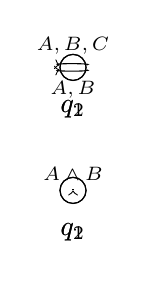
\begin{tikzpicture}[
			transition/.style={above, font=\scriptsize},
		]
		\matrix [column sep=3cm, row sep=0.5cm,
				nodes={circle, draw, minimum size=0.3cm}] {
			\node (q1) [label=below:{$q_1$}] {}; \&
			\node (q2) [label=below:{$q_2$}] {}; \\
			\node (q12) [label=below:{$q_1$}] {}; \&
			\node (q22) [label=below:{$q_2$}] {}; \\
		};
		\draw [->] (q1)
			edge [out=10, in=170] node [transition] {$\set{A, B, C}$} (q2)
			edge [out=-10, in=190] node [transition, below] {$\set{A, B}$} (q2);
		\draw [->] (q12) -- node [transition] {$A \land B$} (q22);
	\end{tikzpicture}
	\caption{Formulae of propositional logic represent a set of arcs.}
	\label{fig:automaton-arcs}
\end{figure}
